
\section{Model Description}

\subsection{Problem Statement}

\begin{figure}[!htb]
	\centering
	\includegraphics[width=0.49\textwidth]{./Figures/Disegno1.eps}
	\caption{Spacecraft with depleting mass and definition of frames and variables}
	\label{fig:Spacecraft}
\end{figure}

The following derivation is a shortened version from Reference\cite{Panicucci:2017fu}. To help define the problem, Figure~\ref{fig:Spacecraft} is displayed. This problem involves a spacecraft consisting of a hub which is a rigid body and has a center of mass location labeled as point $B_c$. The hub has $M$ number of tanks and $N$ number of thrusters attached to it. The figure only shows one tank and one thruster but the analytical development is general. The $i_{\text{th}}$ tank has a center of mass location labeled as $F_{c_i}$ and the $j_{\text{th}}$ thruster is located at $B_j$. The body fixed reference frame $\mathcal{B}$: $\{\bm{\hat{b}}_1\,, \bm{\hat{b}}_2\,,\bm{\hat{b}}_3 \}$ with origin $B$ can be oriented in any direction and point $B$ can be located anywhere fixed to the hub. This means that point $B$ and the center of mass location of the spacecraft, $C$, are not necessarily coincident. As a result, the vector $\bm c$ defines the vector pointing from the body frame origin to the center of mass fo the spacecraft. The inertial reference frame $\mathcal{N}$: $\{\bm{\hat{n}}_1\,, \bm{\hat{n}}_2\,,\bm{\hat{n}}_3 \}$ is centered at $N$ and is fixed in inertial space.
	
	Throughout this paper, vector calculus is used and the notation to define certain quantities needs to be introduced. A position vector, $ \bm{r}_{C/N}$, is the vector pointing from $N$ to $C$. $\bm{\omega}_{\mathcal{B}/\mathcal{N}}$ is the angular velocity of the $\mathcal{B}$ frame with respect to the $\mathcal{N}$ frame.
	$\dot{\bm{r}}$ denotes an inertial time derivate of vector $\bm{r}$ and  $\bm{r}'$ defines a time derivate of $\bm{r}$ with respect to the body frame. Using these definitions, the following describes the Reynolds transport theorem used in this formulation.

\subsection{Equations of Motion}
\subsubsection{Reynolds Transport Theorem and Continuity Equation}
In this section the main tool used for the  development of the governing equations is presented and explained. The Reynolds transport theorem provides a basic tool to pass from a Lagrangian formulation, based on the analysis of particles moving in space, to an Eulerian one, which considers a fixed space volume where physical quantities are exchanged through the boundaries.
\begin{figure}[!htb]
	\centering
	\includegraphics[width=0.49\textwidth]{./Figures/DefSyst.eps}
	\caption{Division of the total system in spacecraft and exhausted gas. The control surface $\mathcal{A}_{\text{sc}}$ represents the exchanging surface between the two subsystems.}
	\label{fig:DefSyst}
\end{figure}
In the present document, the Lagrangian system is labeled $\textit{Body}$, the moving volume of the Eulerian approach is labeled $\mathcal{V}_{\text{sc}}$ and its surface $\mathcal{A}_{\text{sc}}$ are represented in Figure \ref{fig:DefSyst}.

By using this notation, the Reynolds transport theorem affirms:

\begin{equation}
	\frac{^\mathcal{D}\text{d}}{\text{d}t}\int_{\text{Body}} \rho\,\bm{f}\text{d}\mathcal{V} = \frac{^\mathcal{D} \text{d}}{\text{d}\,t}\int_{\mathcal{V}_\text{sc}} \rho\,\bm{f}\text{d}\mathcal{V}  + \int_{\mathcal{A}_\text{sc}} \rho\,\bm{f} \left(\bm{v}_{\text{rel}}\cdot \hat{\bm{n}}\right)\text{d}A
\end{equation}
\noindent
where $\bm{f}$ is a general vectorial quantity transported out from the control volume, $\rho$ is the density of the infinitesimal mass $\text{d}m$, $\hat{\bm{n}}$ the surface normal considered positive if exiting from the control volume, $\mathcal{D}$ is a generic reference frame and $\bm{v}_{\text{rel}}$ is the relative velocity of the particles flowing out from the surface with respect to the control surface itself. This last quantity can be easily defined as $\bm{v}_{\text{rel}}(\bm{x},t) =\displaystyle\frac{^\mathcal{D}\text{d}}{\text{d}t}\bm{r}_{M/B}(\bm{x},t) - \bm{v}_{\text{surf}}(\bm{x},t)$ where $\displaystyle\frac{^\mathcal{D}\text{d}}{\text{d}t}\bm{r}_{M/B}(\bm{x},t)$ is the particles' velocity with respect to the $\mathcal{D}$ frame and $\bm{v}_{\text{surf}}(\bm{x},t)$ is the control surface velocity with respect to the $\mathcal{D}$ reference frame.\newline
Moreover, if the control volume is fixed in the $\mathcal{D}$ frame and a no deformable control volume is considered, the following relation is proved:

\begin{equation}
	\frac{^\mathcal{D}\text{d}}{\text{d}\,t}\int_{\text{Body}} \rho\,\bm{f}\text{d}\mathcal{V} = \int_{\mathcal{V}_\text{sc}} \frac{ ^\mathcal{D}\partial}{\partial\,t}\left(\rho\,\bm{f}\right)\text{d}\mathcal{V}+ \int_{\mathcal{A}_\text{sc}} \rho\,\bm{f} \left(\frac{^\mathcal{D}\text{d}}{\text{d}t}\bm{r}_{M/B}\right)\cdot \hat{\bm{n}}\,\text{d}A
\end{equation}

An additional key equation that is used throughout the paper is the continuity equation. First, the continuity equation is gathered:

\begin{equation}
	\frac{^\mathcal{B}\text{d}}{\text{d}t}\int_{\text{Body}} \rho\, \text{d}m = \frac{^\mathcal{B}\text{d}}{\text{d}t}\int_{\mathcal{V}_\text{sc}} \rho\, \text{d}\mathcal{V} + \int_{\mathcal{A}_\text{sc}} \rho\,\bm{r}'_{M/B} \cdot \hat{\bm{n}}\,\text{d}\mathcal{A}=0
\end{equation}
\noindent
Thus, by defining $\dot{m}_\text{sc} = \frac{^\mathcal{B}\text{d}}{\text{d}t}\int_{\mathcal{V}_\text{sc}} \rho\, \text{d}\mathcal{V}$:

\begin{equation}\label{eq:cambVar}
	\dot{m}_\text{sc} = - \int_{\mathcal{A}_\text{sc}} \rho\,\bm{r}'_{M/B} \cdot \hat{\bm{n}}\,\text{d}\mathcal{A} \qquad \Rightarrow \qquad \text{d}\dot{m} = \rho\,\bm{r}'_{M/B} \cdot \hat{\bm{n}}\,\text{d}\mathcal{A}
\end{equation}
This definition will be used in the derivation of the EOMs. The translational EOM is developed in the following section.

\subsubsection{Translational Equation of Motion}
The derivation of the translational EOM must begins considering Newton's law for a closed system:

\begin{equation}\label{eq:eq3}
	\frac{^{\mathcal{N}}\text{d}}{\text{d}\,t}\int_{\text{Body}}\dot{\bm{r}}_{M/N}\,	\text{d}m= \bm{F}_{\text{ext}}
\end{equation}
where $\dot{\bm{r}}_{M/N}$ is the velocity of the particle at the $M$ point expressed with respect to the inertial reference frame and $\bm{F}_{\text{ext}}$ is the sum of the external forces experienced by the body.

As the total mass of the system is constant, the differentiation operator is brought inside the integration: 
\begin{equation}\label{eq:eq4}
	\frac{^{\mathcal{N}}\text{d}}{\text{d}\,t}\int_{\text{Body}}\dot{\bm{r}}_{M/N}\,	\text{d}m= \int_{\text{Body}}\ddot{\bm{r}}_{M/N}\,\text{d}m
\end{equation}
The acceleration of the origin of the $\mathcal{B}$ frame is expressed as:

\begin{equation}\label{eq:RcRbacc}
	\ddot{\bm{r}}_{M/N} = \ddot{\bm{r}}_{B/N} + \ddot{\bm{r}}_{M/B}
\end{equation}
By using the kinematic transport theorem, the expression of $\ddot{\bm{r}}_{M/B}$ is found:

\begin{equation}\label{eq:rMB_ddot}
	\dot{\bm{r}}_{M/B} = \bm{r}'_{M/B} + \bm{\omega}_{\cal{B}/\cal{N}}\times\bm{r}_{M/B}
\end{equation}
\begin{equation}\label{eq:rMB_dot}
	\ddot{\bm{r}}_{M/B} = \bm{r}''_{M/B}+2\,\bm{\omega}_{\cal{B}/\cal{N}}\times
	\bm{r}'_{M/B} + \dot{\bm{\omega}}_{\cal{B}/\cal{N}}\times \bm{r}_{M/B} + \bm{\omega}_{\cal{B}/\cal{N}}\times\left(\bm{\omega}_{\cal{B}/\cal{N}} \times \bm{r}_{B/M} \right)
\end{equation}

A Lagrangian formulation of the linear momentum equation is deduced by using Equations \eqref{eq:eq3}, \eqref{eq:eq4}, \eqref{eq:RcRbacc} and \eqref{eq:rMB_dot}: 

\begin{multline}\label{eq:eq11}
	\int_{\text{Body}}\left(\ddot{\bm{r}}_{B/N} + \dot{\bm{\omega}}_{\mathcal{B}/\mathcal{N}}\times\bm{r}_{M/B} + \bm{\omega}_{\mathcal{B}/\mathcal{N}} \times\left(\bm{\omega}_{\mathcal{B}/\mathcal{N}} \times\bm{r}_{M/B}\right)\right)\text{d}m +\\+
	2\,\bm{\omega}_{\mathcal{B}/\mathcal{N}}\times\int_{\text{Body}}\bm{r}'_{M/B}\text{d}m + \int_{\text{Body}}\bm{r}''_{M/B}\text{d}m = \bm{F}_{\text{ext}}
\end{multline}

The system mass is constant, therefore the derivative operator can be applied after the integration. This yields:

\begin{equation}	
	\int_{\text{Body}}\bm{r}'_{M/B}\text{d}m = \frac{^{\mathcal{B}}\text{d}}{\text{d}t}\int_{\text{Body}}\bm{r}_{M/B}\text{d}m
\end{equation}
\begin{equation}
	\int_{\text{Body}}\bm{r}''_{M/B}\text{d}m = \frac{^{\mathcal{B}}\text{d}^2}{\text{d}t^2}\int_{\text{Body}}\bm{r}_{M/B}\text{d}m
\end{equation}

By using the Reynolds transport theorem, the two previous equations can be expressed in a space fixed volume, shown in Figure \ref{fig:DefSyst}. Performing this conversion results in the following equations:

\begin{equation}
	\frac{^{\mathcal{B}}\text{d}}{\text{d}t}\int_{\text{Body}}\bm{r}_{M/B} \,\text{d}m = \frac{^{\mathcal{B}} \text{d}}{\text{d}t}\int_{\mathcal{V}_{\text{sc}}} \rho\,\bm{r}_{M/B}\,\text{d}\mathcal{V} + \int_{\mathcal{A}_{\text{sc}}} \rho\,\bm{r}'_{M/B}\cdot\bm{\hat{n}}\,\bm{r}_{M/B}\text{d}A
\end{equation}
\begin{multline}
	\frac{^{\mathcal{B}}\text{d}^2}{\text{d}t^2}\int_{\text{Body}}\bm{r}_{M/B}\, \text{d}m = \frac{^{\mathcal{B}} \text{d}^2}{\text{d}t^2}\int_{\mathcal{V}_{\text{sc}}} \rho\,\bm{r}_{M/B} \,\text{d}\mathcal{V} +\\+ \frac{^{\mathcal{B}} \text{d}}{\text{d}t} \int_{\mathcal{A}_\text{sc}} \rho\,\bm{r}'_{M/B}\cdot\bm{\hat{n}} \,\bm{r}_{M/B}\,\text{d}A + \int_{\mathcal{A}_\text{sc}} \rho\,\bm{r}'_{M/B}\cdot\bm{\hat{n}} \,\bm{r}'_{M/B}\,\text{d}A
\end{multline}
\noindent
where $\bm{v}_{\text{rel}} = \bm{r}' _{M/B}$ because point $B$ is fixed with respect to the spacecraft.  Equation \eqref{eq:eq11} is re-organized by using the previous relations in order to convert it to an Eulerian approach, i.e. based on a volume-based  derivation:

\begin{multline}
	\int_{\text{Body}}\left(\ddot{\bm{r}}_{B/N} + \dot{\bm{\omega}}_{\mathcal{B}/\mathcal{N}}\times\bm{r}_{M/B} + \bm{\omega}_{\mathcal{B}/\mathcal{N}} \times\left(\bm{\omega}_{\mathcal{B}/\mathcal{N}} \times\bm{r}_{M/B}\right)\right)\text{d}m +\\+
	2\,\bm{\omega}_{\mathcal{B}/\mathcal{N}}\times\left(\,\frac{^{\mathcal{B}} \text{d}}{\text{d}t}\int_{\mathcal{V}_{\text{sc}}} \rho\,\bm{r}_{M/B}\,\text{d}\mathcal{V} + \int_{\mathcal{A}_{\text{sc}}} \rho\,\bm{r}'_{M/B}\cdot\bm{\hat{n}}\,\bm{r}_{M/B}\text{d}A\right) \;+ 	 \frac{^{\mathcal{B}} \text{d}^2}{\text{d}t^2}\int_{\mathcal{V}_{\text{sc}}} \rho\,\bm{r}_{M/B} \,\text{d}\mathcal{V} +\\+ \frac{^{\mathcal{B}} \text{d}}{\text{d}t} \int_{\mathcal{A}_\text{sc}} \rho\,\bm{r}'_{M/B}\cdot\bm{\hat{n}} \,\bm{r}_{M/B}\,\text{d}A + \int_{\mathcal{A}_\text{sc}} \rho\,\bm{r}'_{M/B}\cdot\bm{\hat{n}} \,\bm{r}'_{M/B}\,\text{d}A  
	= \bm{F}_{\text{ext}}
\end{multline} 

As explained in previous work, if all of the mass is contained in the control volume at the initial time, then a particular relation results because no mass is outside the control volume at $t=0$ and the dynamic quantities will be transported out during the integration. This relationship is quantified in the following equation:

\begin{multline}
	\bm{F}_{\text{ext}} - \int_{\text{Body}}\left(\ddot{\bm{r}}_{B/N} + \dot{\bm{\omega}}_{\mathcal{B}/\mathcal{N}}\times\bm{r}_{M/B} + \bm{\omega}_{\mathcal{B}/\mathcal{N}} \times\left(\bm{\omega}_{\mathcal{B}/\mathcal{N}} \times\bm{r}_{M/B}\right)\right)\text{d}m 
	= \int_{\mathcal{V}_{\text{sc}}} \text{d}\bm{F}_{\text{vol}}+\\ +\int_{\mathcal{A}_{\text{sc}}} \text{d}\bm{F}_{\text{surf}} - \int_{\mathcal{V}_{\text{sc}}}\rho\,\left(\ddot{\bm{r}}_{B/N} + \dot{\bm{\omega}}_{\mathcal{B}/\mathcal{N}}\times\bm{r}_{M/B} + \bm{\omega}_{\mathcal{B}/\mathcal{N}} \times\left(\bm{\omega}_{\mathcal{B}/\mathcal{N}} \times\bm{r}_{M/B}\right)\right)\text{d}\mathcal{V}
\end{multline}  
\noindent
where the forces are divided into volumetric forces and the forces applied on the spacecraft surface. Rearranging this result, replacing the definition of $\bm{F}_{\text{ext}}$, and isolating the forces to the right hand side of the equation yields:
\begin{multline}\label{eq:ComplTranslEOM}
	\int_{\mathcal{V}_{\text{sc}}}\rho\,\left(\ddot{\bm{r}}_{B/N} + \dot{\bm{\omega}}_{\mathcal{B}/\mathcal{N}}\times\bm{r}_{M/B} + \bm{\omega}_{\mathcal{B}/\mathcal{N}} \times\left(\bm{\omega}_{\mathcal{B}/\mathcal{N}} \times\bm{r}_{M/B}\right)\right)\text{d}\mathcal{V} +\\+
	2\,\bm{\omega}_{\mathcal{B}/\mathcal{N}}\times\left(\,\frac{^{\mathcal{B}} \text{d}}{\text{d}t}\int_{\mathcal{V}_{\text{sc}}} \rho\,\bm{r}_{M/B}\,\text{d}\mathcal{V}\; + \int_{\mathcal{A}_{\text{sc}}} \rho\,\bm{r}'_{M/B}\cdot\bm{\hat{n}}\,\bm{r}_{M/B}\text{d}A\right) \;+ 	 \frac{^{\mathcal{B}} \text{d}^2}{\text{d}t^2}\int_{\mathcal{V}_{\text{sc}}} \rho\,\bm{r}_{M/B} \,\text{d}\mathcal{V} +\\+ \frac{^{\mathcal{B}} \text{d}}{\text{d}t} \int_{\mathcal{A}_\text{sc}} \rho\,\bm{r}'_{M/B}\cdot\bm{\hat{n}} \,\bm{r}_{M/B}\,\text{d}A + \int_{\mathcal{A}_\text{sc}} \rho\,\bm{r}'_{M/B}\cdot\bm{\hat{n}} \,\bm{r}'_{M/B}\,\text{d}A  
	= \int_{\mathcal{V}_{\text{sc}}} \text{d}\bm{F}_{\text{vol}} +\int_{\mathcal{A}_{\text{sc}}} \text{d}\bm{F}_{\text{surf}}
\end{multline}

One goal for this paper is to develop the EOMs of a spacecraft with depleting mass without the necessity of continuing to track the depleted mass once it has left the spacecraft. One aspect of achieving this goal, is to define the center of mass of the spacecraft with respect to point $B$, including the remaining fuel while disregarding the spent fuel. This variable, $\bm{c} = \bm{r}_{C/B}$, is defined as:
\begin{equation}\label{eq:def_rCB}
	\bm{c}=\frac{m_{\text{hub}}\,\bm{r}_{Bc/B} + \sum_{i=1}^{M}m_{\text{fuel}_i}\,\bm{r}_{Fc_i/B}}{m_{\text{hub}}+ \sum_{i=1}^{M}m_{\text{fuel}_i}}
\end{equation}
where $m_{\text{hub}}$ is the mass of the hub, $m_{\text{fuel}_i}$ is the i-th tank's fuel mass and $\bm{r}_{Fc_i/B}$ is the position of the center of mass of the i-th tank's fuel.
In order to infer the influence of the mass variation in the EOMs equation of motion the first and second time derivatives with respect to the body frame of $\bm c$ is defined:

\begin{multline}\label{eq:eq17}
	\bm{c}' = \frac{\sum_{i=1}^{M}\left(\dot{m}_{\text{fuel}_i}\bm{r}_{Fc_i/B} + m_{\text{fuel}_i}\bm{r}'_{Fc_i/B}\right)}{m_{\text{hub}}+ \sum_{i=1}^{M}m_{\text{fuel}_i}} + \vspace{5pt}\\
	- \frac{\left(\sum_{i=1}^{M}\dot{m}_{\text{fuel}_i}\right)\left(m_{\text{hub}}\,\bm{r}_{Bc/B} + \sum_{i=1}^{M}m_{\text{fuel}_i}\,\bm{r}_{Fc_i/B}\right)}{\left(m_{\text{hub}}+ \sum_{i=1}^{M}m_{\text{fuel}_i}\right)^2}
\end{multline}

\begin{multline}\label{eq:eq18}
	\bm{c}'' = \frac{\sum_{i=1}^{M}\left(\ddot{m}_{\text{fuel}_i}\bm{r}_{Fc_i/B} +2\,\dot{m}_{\text{fuel}_i}\bm{r}'_{Fc_i/B}+ m_{\text{fuel}_i}\bm{r}''_{Fc_i/B}\right)}{m_{\text{hub}}+ \sum_{i=1}^{M}m_{\text{fuel}_i}} + \vspace{5pt}\\
	- \frac{\left(\sum_{i=1}^{M}\ddot{m}_{\text{fuel}_i}\right)\left(m_{\text{hub}}\,\bm{r}_{Bc/B} + \sum_{i=1}^{M}m_{\text{fuel}_i}\,\bm{r}_{Fc_i/B}\right)  }{\left(m_{\text{hub}}+ \sum_{i=1}^{M}m_{\text{fuel}_i}\right)^2} +\\-
	\frac{2\,\left(\sum_{i=1}^{M}\dot{m}_{\text{fuel}_i}\right)\sum_{i=1}^{M}\left(\dot{m}_{\text{fuel}_i}\bm{r}_{Fc_i/B} + m_{\text{fuel}_i}\bm{r}'_{Fc_i/B}\right) }{\left(m_{\text{hub}}+ \sum_{i=1}^{M}m_{\text{fuel}_i}\right)^2} +\\
	+ \frac{2\,\left(\sum_{i=1}^{M}\dot{m}_{\text{fuel}_i}\right)^2\left(m_{\text{hub}}\bm{r}_{Bc/B} +\sum_{i=1}^{M} m_{\text{fuel}_i}\bm{r}_{Fc_i/B}\right)}{\left(m_{\text{hub}}+ \sum_{i=1}^{M}m_{\text{fuel}_i}\right)^3}
\end{multline}
Using these definitions of $\bm c$, the translational EOM can be simplified. Additionally, some assumptions need to be defined to further simplify the translational EOM. The hub is assumed to be rigid, therefore deformations are not considered. The mass flow within the tanks and the thrusters is assumed to be a second order effect and ignored for this paper. The particles are assumed to be accelerated instantaneously from the spacecraft velocity, $\dot{\bm{r}}_{B/N}$, to the exhausted velocity $\bm{v}_{\text{exh}}$ at the nozzle. And the exhausted velocity $\bm{v}_{\text{exh}}$ is considered constant and parallel to the nozzle's normal $\hat{\bm{n}}$.

The first integral in Eqn. \eqref{eq:ComplTranslEOM} is computed using the fact that $\bm{r}_{M/B} = \bm{c} + \bm{r}_{M/C}$ and the result is shown in the following equation:

\begin{multline}\label{eq:eq19}
	\int_{\mathcal{V}_{\text{sc}}}\rho\,\left(\ddot{\bm{r}}_{B/N} + \dot{\bm{\omega}}_{\mathcal{B}/\mathcal{N}}\times\bm{r}_{M/B} + \bm{\omega}_{\mathcal{B}/\mathcal{N}} \times\left(\bm{\omega}_{\mathcal{B}/\mathcal{N}} \times\bm{r}_{M/B}\right)\right)\text{d}\mathcal{V} = \\=
	m_{\text{sc}} \,\bm{\ddot{r}}_{B/N} + m_{\text{sc}}\,\bm{\dot{\omega}}_{\mathcal{B}/\mathcal{N}} \times\bm{c} + m_{\text{sc}}\,\bm{\omega}_{\mathcal{B}/\mathcal{N}} \times\left(\bm{\omega}_{\mathcal{B}/\mathcal{N}}\times\bm{c}\right) 
\end{multline}
\noindent 
where $m_{\text{sc}}=m_{\text{hub}}+ \sum_{i=1}^{M}m_{\text{fuel}_i}$ is the instantaneous mass of the spacecraft. The second and fourth integrals are computed and yield:

\begin{equation}\label{eq:eq20}
	\frac{^{\mathcal{B}} \text{d}}{\text{d}t}\int_{\mathcal{V}_{\text{sc}}} \rho\,\bm{r}_{M/B}\,\text{d}\mathcal{V} = \frac{^{\mathcal{B}} \text{d}}{\text{d}t}\left(m_{\text{sc}}\,\bm{c}\right) = m_{\text{sc}}\,\bm{c}' + \dot{m}_{\text{fuel}}\bm{c}
\end{equation}
\begin{equation}\label{eq:eq21}
	\frac{^{\mathcal{B}} \text{d}^2}{\text{d}t^2}\int_{\mathcal{V}_{\text{sc}}} \rho\,\bm{r}_{M/B} \,\text{d}\mathcal{V} = \frac{^{\mathcal{B}} \text{d}^2}{\text{d}t^2} \left(m_{\text{sc}}\,\bm{c}\right) = m_{\text{sc}}\,\bm{c}'' + 2\,\dot{m}_{\text{fuel}}\,\bm{c}' + \ddot{m}_{\text{fuel}}\bm{c}
\end{equation}
where $\dot{m}_{\text{fuel}} = \sum_{i=1}^{M}\dot{m}_{\text{fuel}_i}$ and $\ddot{m}_{\text{fuel}} = \sum_{i=1}^{M}\ddot{m}_{\text{fuel}_i}$.

In order to find the term calculated on the reference surface seen in the third, fifth and sixth integrals,  it is convenient to separate the integrals on the surface of each nozzle. Moreover, as the fuel's properties are flowing out of a surface plane, it is convenient to consider that  $\bm{r}_{M/B} = \bm{r}_{M/Fc_j}+ \bm{r}_{Fc_j/B} $ where $Fc_i$ is the area's geometric center. Finally, an appropriate variable transformation is given in Eqn. \eqref{eq:cambVar}. Performing these calculations on the third integral results in:
\begin{equation}\label{eq:eq22}
	\int_{\mathcal{A}_{\text{sc}}} \rho\,\bm{r}'_{M/B}\cdot\bm{\hat{n}}\,\bm{r}_{M/B}\,\text{d}A =-\sum_{j=1}^{N} \int_{\dot{m}_{\text{noz}_j}}\left(\bm{r}_{M/N_j}+ \bm{r}_{N_j/B}\right)\text{d}\dot{m}  =-\sum_{j=1}^{N}\dot{m}_{\text{noz}_j}\bm{r}_{N_j/B}
\end{equation}
\noindent
where the first part of the integral is null because of barycenter definition and $\dot{m}_{\text{noz}_j}$ is the mass flow of the $j-$th nozzle. The fifth integral in Eq.~\eqref{eq:ComplTranslEOM} yields:
\begin{equation}\label{eq:eq23}
	\frac{^{\mathcal{B}} \text{d}}{\text{d}t} \int_{\mathcal{A}_\text{sc}} \rho\,\bm{r}'_{M/B}\cdot\bm{\hat{n}} \,\bm{r}_{M/B}\,\text{d}A = \frac{^{\mathcal{B}} \text{d}}{\text{d}t} \left(-\sum_{j=1}^{N}\dot{m}_{\text{noz}_j}\bm{r}_{N_j/B}\right) = -\sum_{j=1}^{N}\ddot{m}_{\text{noz}_j}\bm{r}_{N_j/B}
\end{equation}
\noindent
Using the assumption introduced earlier in this section, $\bm{r}'_{M/B} = \bm{v}_{\text{exh}}$, the sixth is integral is found and can be in the following equation:

\begin{equation}\label{eq:eq24}
	\int_{\mathcal{A}_\text{sc}} \rho\,\bm{r}'_{M/B}\cdot\bm{\hat{n}} \,\bm{r}'_{M/B} \,\text{d}A  =\sum_{j=1}^{N}\int_{\mathcal{A}_{\text{noz}_j}}\rho\,\bm{r}'_{M/B}\cdot\bm{n}\,\bm{r}'_{M/B}\text{d}A = -\sum_{j=1}^{N}\dot{m}_{\text{noz}_j}\,\bm{v}_{\text{exh}_j}
\end{equation}
\noindent
where $\bm{v}_{\text{exh}_j}$ is the exhausted velocity of a particle exiting from the $j-$th nozzle.

The two integrals on the right-hand-side of Eq.~\eqref{eq:ComplTranslEOM} depends on the force model chosen. Therefore, to not lose generality, the resulting surface integral due to the pressure jump between the nozzle and the environment is the only term that is analytically computed seen in the following equation:

\begin{equation}\label{eq:eq25}
	\int_{\mathcal{V}_{\text{sc}}} \text{d}\bm{F}_{\text{vol}} +\int_{\mathcal{A}_{\text{sc}}} \text{d}\bm{F}_{\text{surf}} = \bm{F}_{\text{ext, vol}} + \bm{F}_{\text{ext, surf}} + \sum_{j=1}^{N}\frac{\bm{v}_{\text{exh}_j}}{v_{\text{exh}_j}}\,A_{\text{noz}_j}\,(p_{\text{exh}_j} - p_{\text{atm}})
\end{equation}
\noindent
where $\bm{F}_{\text{ext, vol}}$ are the external forces acting on the control volume, $\bm{F}_{\text{ext, surf}}$ are the external forces accelerating the control surface, $p_{\text{exh}_j}$ is the particles' exhausted pressure at the $j-$th nozzle and  $p_{\text{atm}}$ is the atmospheric pressure.

Finally, Equation \eqref{eq:ComplTranslEOM} is rewritten considering the nozzles' geometry and fluid properties by using Equations~\eqref{eq:eq20}-~\eqref{eq:eq25}:
\begin{multline}
	m_{\text{sc}} \bm{\ddot{r}}_{B/N} + m_{\text{sc}}\,\bm{\dot{\omega}}_{\mathcal{B}/\mathcal{N}} \times\bm{c} + m_{\text{sc}}\,\bm{\omega}_{\mathcal{B}/\mathcal{N}} \times\left(\bm{\omega}_{\mathcal{B}/\mathcal{N}}\times\bm{c}\right) + m_{\text{sc}}\,\bm{c}'' + 2\,\dot{m}_{\text{fuel}}\,\bm{c}' +\\+ \ddot{m}_{\text{fuel}}\bm{c} + 2\,\bm{\omega}_{\mathcal{B}/\mathcal{N}} \times \bigg(m_{\text{sc}}\,\bm{c}'+ \dot{m}_{\text{fuel}}\bm{c} - \sum_{j=1}^{N}\dot{m}_{\text{noz}_j}\bm{r}_{N_j/B}  \bigg) - \sum_{j=1}^{N}\ddot{m}_{\text{noz}_j}\bm{r}_{N_j/B}	+\\-
	\sum_{j=1}^{N}\dot{m}_{\text{noz}_j}\,\bm{v}_{\text{exh}_j} = \bm{F}_{\text{ext, vol}} + \bm{F}_{\text{ext, surf}} + \sum_{j=1}^{N}\frac{\bm{v}_{\text{exh}_j}}{v_{\text{exh}_j}}\,A_{\text{noz}_j}\,(p_{\text{exh}_j} - p_{\text{atm}})
\end{multline}
The previous equation is modified by defining the following quantity:

\begin{equation}\label{eq:IspRel}
	\bm{F}_{\text{thr}_j}= \bm{v}_{\text{exh}_j}\,\left(\frac{A_{\text{noz}_j}}{v_{\text{exh}_j}}\,(p_{\text{exh}_j} - p_{\text{atm}}) + \dot{m}_{\text{noz}_j}\right) = I_{\text{sp}_j}\,g_0\,\dot{m}_{\text{noz}_j}\frac{\bm{v}_{\text{exh}_j}}{v_{\text{exh}_j}}
\end{equation}

For further simplicity, the cross product is substituted with the associated skew symmetric matrix, and the translational equation is written in a more compact form:

\begin{multline}\label{eq:eq29}
	\ddot{\bm{r}}_{B/N} + \left[\tilde{\bm{c}}\right]^T\dot{\bm{\omega}}_{\cal{B}/\cal{N}} =  \frac{\bm{F}_{\text{thr}}}{m_{\text{sc}}} - 2\,\frac{\dot{m}_{\text{fuel}}}{m_{\text{sc}}}\,\left(c' + \left[\tilde{\bm{\omega}}_{\cal{B}/\cal{N}}\right]\times\bm{c}\right) - \bm{c}''+2\,\left[\tilde{\bm{\omega}}_{\cal{B}/\cal{N}}\right]^T
	\bm{c}'\\- \ddot{m}_{\text{fuel}}\,\bm{c} + \left[\tilde{\bm{\omega}}_{\cal{B}/\cal{N}}\right]^T \left[\tilde{\bm{\omega}}_{\cal{B}/\cal{N}}\right] \bm{c} +\frac{2}{m_{\text{sc}}}\sum_{j=1}^{N}\dot{m}_{\text{noz}_j} \left[\tilde{\bm{\omega}}_{\cal{B}/\cal{N}}\right] \bm{r}_{N_j/B}
	\\+ \frac{	1}{m_{\text{sc}}} \sum_{j=1}^{N}\ddot{m}_{\text{noz}_j}\bm{r}_{Fc_j/B}  +\frac{\bm{F}_{\text{ext, vol}}}{m_{\text{sc}}}  + \frac{\bm{F}_{\text{ext, surf}}}{m_{\text{sc}}} 
\end{multline}
Multiplying my 

\begin{multline}\label{eq:eq30}
m_{\text{sc}} \ddot{\bm{r}}_{B/N} - m_{\text{sc}} \left[\tilde{\bm{c}}\right]\dot{\bm{\omega}}_{\cal{B}/\cal{N}} =  \bm{F}_{\text{thr}} - 2\,\dot{m}_{\text{fuel}} \left(c' + \left[\tilde{\bm{\omega}}_{\cal{B}/\cal{N}}\right]\times\bm{c}\right) - m_{\text{sc}} \bm{c}''-2 m_{\text{sc}} \,\left[\tilde{\bm{\omega}}_{\cal{B}/\cal{N}}\right]
\bm{c}'\\- m_{\text{sc}} \ddot{m}_{\text{fuel}}\,\bm{c} - m_{\text{sc}} \left[\tilde{\bm{\omega}}_{\cal{B}/\cal{N}}\right] \left[\tilde{\bm{\omega}}_{\cal{B}/\cal{N}}\right] \bm{c} +2 \sum_{j=1}^{N}\dot{m}_{\text{noz}_j} \left[\tilde{\bm{\omega}}_{\cal{B}/\cal{N}}\right] \bm{r}_{N_j/B}
\\+ \sum_{j=1}^{N}\ddot{m}_{\text{noz}_j}\bm{r}_{Fc_j/B}  +\bm{F}_{\text{ext, vol}} + \bm{F}_{\text{ext, surf}}
\end{multline}
This EOM is the translational equation for an open system subjected to external forces $\bm{F}_{\text{ext, vol}} \text{ and } \bm{F}_{\text{ext, surf}}$ and thrust $\bm{F}_{\text{thr}}=\sum_{j=1}^{N}\bm{F}_{\text{thr}_j}$ due to mass depletion of the spacecraft, represented in Figure \ref{fig:Spacecraft}.
From this equation, it can be deduced that the variation of the mass inside the spacecraft directly impacts the position of the satellite with respect to the origin as the body fixed point $B$ changes its state of motion according to the variation of the tanks' linear inertia. In the next section, the rotational EOM for the spacecraft is developed.

\subsubsection{Rotational Equation of Motion}
The goal of this section is to develop the EOM associated with attitude dynamics of a spacecraft with depleting mass due to thrusters pulling mass from fuel tanks. Beginning from Newton's equation:

\begin{equation}
	\ddot{\bm{r}}_{M/N}\,\text{\text{d}}m=\text{d}\bm{F} \quad \Rightarrow \quad
	\bm{r}_{M/N} \times \ddot{\bm{r}}_{M/N}\,\text{d}m =\bm{r}_{M/N} \times \text{d}\bm{F}
\end{equation}
and performing an integration over the system:

\begin{equation}
	\int_{\text{Body}} \bm{r}_{M/N} \times \ddot{\bm{r}}_{M/N}\,\text{d}m = \int_{\text{Body}}\bm{r}_{M/N} \times \text{d}\bm{F}
\end{equation}
The term on the left-hand side of the previous equation is manipulated in order to define the momentum about point $B$. This manipulation can be seen in the following equation:

\begin{multline}\label{eq:eq32}
	\int_{\text{Body}} \rho\,\bm{r}_{M/N} \times \ddot{\bm{r}}_{M/N}\,\text{d}\mathcal{V} = \int_{\text{Body}} \rho\,\bm{r}_{M/B} \times \ddot{\bm{r}}_{M/B}\,\text{d}\mathcal{V} +\\ + \int_{\text{Body}} \rho\,\bm{r}_{B/N} \times \ddot{\bm{r}}_{M/N}\,\text{d}\mathcal{V} + \int_{\text{Body}} \rho\,\bm{r}_{M/B} \times \ddot{\bm{r}}_{B/N}\,\text{d}\mathcal{V} = \int_{\text{Body}}\bm{r}_{M/N} \times \text{d}\bm{F}
\end{multline}
Knowing that $\ddot{\bm{r}}_{M/N}\,\text{\text{d}}m=\text{d}\bm{F}$, the torque caused by the forces acting on the body is  easily defined:

\begin{equation}
	\int_{\text{Body}}\bm{r}_{M/N} \times \text{d}\bm{F}-\int_{\text{Body}}  \rho\,\bm{r}_{B/N} \times \ddot{\bm{r}}_{M/N}\,\text{d}\mathcal{V} 
	= \int_{\text{Body}} \left(\bm{r}_{M/N}-\bm{r}_{B/N}\right) \times \text{d}\bm{F} = \bm{L}_{B}
\end{equation}
\noindent
where $\bm{L}_{B}$ is the torque with respect to the body-fixed point $B$.

As the mass of the system is constant, the derivative of the angular momentum about point $B$ is inferred from Equation~\eqref{eq:eq32} due to a property of the cross product and the previously explained Reynold's transport theorem:

\begin{multline}
	\int_{\text{Body}}  \rho\,\bm{r}_{M/B} \times \ddot{\bm{r}}_{M/B}\,\text{d}\mathcal{V}  = \frac{^\mathcal{N}\text{d}}{\text{d}t} \int_{\mathcal{V}_{\text{sc}}} \rho\,\bm{r}_{M/B} \times \dot{\bm{r}}_{M/B}\,\text{d}\mathcal{V} + \int_{\mathcal{A}_{\text{sc}}} \rho\,\bm{r}'_{M/B} \cdot\bm{\hat{n}} \left(\bm{r}_{M/B} \times \dot{\bm{r}}_{M/B}\right)\text{d}A
\end{multline} 

Moreover, similar to the translational equation, if all the mass of the system is assumed to be contained inside the control volume at the initial time, the following relationship results:

\begin{multline}
	\int_{\text{Body}} \rho\,\bm{r}_{M/B} \times \ddot{\bm{r}}_{B/N}\,\text{d}\mathcal{V} -  \bm{L}_{B}=  \int_{\mathcal{V}_{\text{sc}}} \rho\,\bm{r}_{M/B} \times \ddot{\bm{r}}_{B/N}\,\text{d}\mathcal{V} -  \int_{\mathcal{V}_{\text{sc}}}\bm{r}_{M/B} \times \text{d}\bm{F}_{\text{vol}} +\\- \int_{\mathcal{A}_{\text{sc}}} \bm{r}_{M/B} \times\text{d}\bm{F}_{\text{surf}} = {m}_{\text{sc}} \bm{c} \times \ddot{\bm{r}}_{B/N}-\bm{L}_{B,\,\text{vol}}-\bm{L}_{B,\,\text{surf}}
\end{multline}
\noindent
where $\bm{L}_{B,\,\text{vol}}\text{ and }\bm{L}_{B,\,\text{surf}}$ are the torques caused by the volume and surface forces about point $B$. The general rotational equation for a control volume in a rotating reference frame is reorganized:

\begin{multline}\label{eq:eq36}
	\dot{\bm{H}}_{\text{sc, }B} + \int_{\mathcal{A}_{\text{sc}}} \rho\,\bm{r}'_{M/B} \cdot\bm{\hat{n}} \left(\bm{r}_{M/B} \times \dot{\bm{r}}_{M/B}\right)\text{d}A +{m}_{\text{sc}} \bm{c} \times \ddot{\bm{r}}_{B/N}=\bm{L}_{B,\,\text{vol}}+\bm{L}_{B,\,\text{surf}}
\end{multline}

To perform the inertial derivative of $\bm{H}_{\text{sc, }B}$, first the definition of $\bm{H}_{\text{sc, }B}$ is defined:
\begin{multline}
	\bm{H}_{\text{sc, }B}= \left[I_{\text{hub},\,B_c}\right] \bm{\omega}_{\cal{B}/\cal{N}} + \bm{r}_{Bc/B} \times m_\text{hub} \,\dot{\bm{r}}_{Bc/B} +\\ +\sum_{i=1}^{M}\left(\left[I_{\text{fuel}_i,\,Fc_i}\right]\, \bm{\omega}_{\cal{B}/\cal{N}} + \bm{r}_{Fc_i/B} \times m_{\text{fuel}_i}\, \dot{\bm{r}}_{Fc_i/B}\right)
\end{multline}
where $\left[I_{\text{hub},\,B_c}\right]$ is the hub's inertia about its center of mass, $B_c$, and $\left[I_{\text{fuel}_i,\,Fc_i}\right]$ is the $i-$th tank's inertia about its center of mass, $Fc_i$. Furthermore, an analytical expression of mass depletion in the rotational motion is deduced:
\begin{multline}\label{eq:HscB_dot}
	\dot{\bm{H}}_{\text{sc, }B} = \left[I_{\text{hub},\,Bc}\right]\dot{\bm{\omega}}_{\cal{B}/\cal{N}} + \bm{\omega}_{\cal{B}/\cal{N}} \times \left(\left[I_{\text{hub},\,Bc}\right]\bm{\omega}_{\cal{B}/\cal{N}}\right)+ \bm{r}_{Bc/B} \times m_\text{hub}\,\ddot{\bm{r}}_{Bc/B} +\\
	+ \sum_{i=1}^{M}\left(\left[I_{\text{fuel}_i,\,Fc_i}\right] \dot{\bm{\omega}}_{\cal{B}/\cal{N}} + \bm{\omega}_{\cal{B}/\cal{N}} \times \left(\left[I_{\text{fuel}_i,\,Fc_i}\right]\, \bm{\omega}_{\cal{B}/\cal{N}}\right) 
	+ \bm{r}_{Fc_i/B} \times m_{\text{fuel}_i}\, \ddot{\bm{r}}_{Fc_i/B}+\right.\\ 
	\left.+ \bm{r}_{Fc_i/B} \times \dot{m}_{\text{fuel}_i} \,\dot{\bm{r}}_{Fc_i/B} + \left[I_{\text{fuel}_i,\, Fc_i}\right]' \, \bm{\omega}_{\cal{B}/\cal{N}}\right)
\end{multline}

It should be noted here that any relative motion of particles inside the fuel tanks of the spacecraft has been neglected and, as a consequence, the effects both of the Coriolis' acceleration and of the whirling motion of the fuel on the spacecraft dynamics have not been considered.

Additionally, the inertial time derivate of the vectors $\bm{r}_{Bc/B}$ and $\bm{r}_{Fc_i/B}$ is computed using the transport theorem between the two reference frames given in Equations \eqref{eq:rMB_ddot} and \eqref{eq:rMB_dot} and, considering that the point $B_c$ is fixed in the $\mathcal{B}$ frame, Equation \eqref{eq:HscB_dot} is rewritten:

\begin{multline}\label{eq:HscB_complic}
	\dot{\bm{H}}_{\text{sc, }B} = \left[I_{\text{hub},\,Bc}\right]\dot{\bm{\omega}}_{\cal{B}/\cal{N}} + \bm{\omega}_{\cal{B}/\cal{N}} \times \left(\left[I_{\text{hub},\,Bc}\right]\bm{\omega}_{\cal{B}/\cal{N}}\right) 
	+ \bm{r}_{Bc/B} \times m_\text{hub}\,\left(\dot{\bm{\omega}}_{\cal{B}/\cal{N}} \times \bm{r}_{Bc/B} +\right.\\
	+\left. \bm{\omega}_{\cal{B}/\cal{N}} \times \left(\bm{\omega}_{\cal{B}/\cal{N}} \times \bm{r}_{Bc/B}\right) \right) 
	+\sum_{i=1}^{M} \bigl(\left[I_{\text{fuel}_i,\,Fc_i}\right] \dot{\bm{\omega}}_{\cal{B}/\cal{N}} + \bm{\omega}_{\cal{B}/\cal{N}} \times \left(\left[I_{\text{fuel}_i,\,Fc_i}\right] \bm{\omega}_{\cal{B}/\cal{N}}\right) +\\ 
	+ \bm{r}_{Fc_i/B} \times m_{\text{fuel}_i}\, \bigl( \bm{r}''_{Fc_i/B} + 2\,\bm{\omega}_{\mathcal{B}/\mathcal{N}} \times \bm{r}'_{Fc_i/B}
	+ \dot{\bm{\omega}}_{\cal{B}/\cal{N}} \times \bm{r}_{Fc_i/B} + \bm{\omega}_{\cal{B}/\cal{N}} \times
	\left(\bm{\omega}_{\cal{B}/\cal{N}} \times \bm{r}_{Fc_i/B}\right) \bigr)+\\ 
	+
	\bm{r}_{Fc_i/B} \times \dot{m}_{\text{fuel}_i} \,\left(\bm{r}'_{Fc_i/B}+\bm{\omega}_{\cal{B}/\cal{N}} \times \bm{r}_{Fc_i/B}\right) 
	+ \left[I_{\text{fuel,}_i,\,Fc_i}\right]' \, \bm{\omega}_{\cal{B}/\cal{N}}\bigr)
\end{multline}

In order to simplify compact Equation \eqref{eq:HscB_complic} the following inertia matrices are defined using the skew symmetric matrix to replace the cross product:
\begin{equation}\label{eq:eq44}
	\left[I_{\text{hub},\,B}\right]= \left[I_{\text{hub},\,Bc}\right] + m_\text{hub}\, \left[\tilde{\bm{r}}_{Bc/B}\right]\left[\tilde{\bm{r}}_{Bc/B}\right]^T 
\end{equation}
\begin{equation}\label{eq:eq45}
	\left[I_{\text{fuel}_i,\,B}\right]= \left[I_{\text{fuel}_i,\,Fc_i}\right] + m_{\text{fuel}_i}\, \left[\tilde{\bm{r}}_{Fc_i/B}\right]\left[\tilde{\bm{r}}_{Fc_i/B}\right]^T
\end{equation}
\begin{equation}\label{eq:eq46}
	\left[I_{\text{sc, }B}\right]=  \left[I_{\text{hub},\,B}\right] + \sum_{i=1}^{M}\left[I_{\text{fuel}_i,\,B}\right]
\end{equation}
Moreover, using the Jacobi identity for the cross product $
\mathbf {a} \times (\mathbf {b} \times \mathbf {c} )+\mathbf {b} \times (\mathbf {c} \times \mathbf {a} )+\mathbf {c} \times (\mathbf {a} \times \mathbf {b} )=\mathbf {0}$, the body relative time derivative of the fuel inertia in the $\mathcal{B}$ reference frame is introduced:

\begin{multline}\label{eq:eq47}
	\bm{r}_{Fc_i/B} \times \left(2\,\bm{\omega}_{\mathcal{B}/\mathcal{N}} \times \bm{r}'_{Fc_i/B}\right) =-\bm{r}_{Fc_i/B} \times \left( \bm{r}'_{Fc_i/B} \times \bm{\omega}_{\mathcal{B}/\mathcal{N}}\right) 
	+\\-\bm{r}'_{Fc_i/B} \times \left( \bm{r}_{Fc_i/B} \times \bm{\omega}_{\mathcal{B}/\mathcal{N}}\right) + \bm{\omega}_{\mathcal{B}/\mathcal{N}} \times \left(\bm{r}_{Fc_i/B}\times \bm{r}'_{Fc_i/B}\right)
\end{multline}
\begin{multline}\label{eq:eq48}
	\left[I_{\text{fuel}_i,\,B}\right]'= \left[I_{\text{fuel}_i,\,Fc_i}\right] + \dot{m}_{\text{fuel}_i}\, \left[\tilde{\bm{r}}_{Fc_i/B}\right]\left[\tilde{\bm{r}}_{Fc_i/B}\right]^T +\\+ m_{\text{fuel}_i}\, \left(\left[\tilde{\bm{r}}_{Fc_i/B}\right]\left[\tilde{\bm{r}}'_{Fc_i/B}\right]^T+ \left[\tilde{\bm{r}}'_{Fc_i/B}\right]\left[\tilde{\bm{r}}_{Fc_i/B}\right]^T\right)
\end{multline}
By substituting Equations \eqref{eq:eq44}-\eqref{eq:eq48} Eq.\eqref{eq:HscB_complic} is simplified to:
\begin{multline}\label{eq:eq49}
	\dot{\bm{H}}_{\text{sc, }B} = \left[I_{\text{sc, }B}\right]\,\dot{\bm{\omega}}_{\cal{B}/\cal{N}} + \left[\tilde{\bm{\omega}}_{\cal{B}/\cal{N}}\right]\left[I_{\text{sc, }B}\right]\,\bm{\omega}_{\cal{B}/\cal{N}} + \sum_{i=1}^{M}\left(m_{\text{fuel}_i}\,\left[\tilde{\bm{r}}_{Fc_i/B}\right] \bm{r}''_{Fc_i/B} +\right. \\
	\left.+ \dot{m}_{\text{fuel}_i} \left[\tilde{\bm{r}}_{Fc_i/B}\right]\bm{r}'_{Fc_i/B}+ \left[I_{\text{fuel}_i,\,B}\right]' \, \bm{\omega}_{\cal{B}/\cal{N}}
	+ \left[\tilde{\bm{\omega}}_{\mathcal{B}/\mathcal{N}}\right] \left[\tilde{\bm{r}}_{Fc_i/B}\right] \bm{r}'_{Fc_i/B}\right)
\end{multline}

Considering that at the nozzles's exit, $\dot{\bm{r}}_{M/B} = \bm{v}_{exh_j} + \bm{\omega}_{\cal{B}/\cal{N}} \times \bm{r}_{M/B}$ and $\text{d}\dot{m} =- \rho\,\bm{r}_{M/B}'\cdot\hat{\bm{n}} \,\text{d}A$, the surface integral is expressed in terms of the nozzles' surface:
\begin{multline}\label{eq:eq50}
	\int_{A_{\text{exh}}} \rho\,\bm{r}'_{M/B}\cdot\bm{n} \left(\bm{r}_{M/B} \times \dot{\bm{r}}_{M/B}\right)\text{d}A =- \sum_{j=1}^{N}\int_{\dot{m}_{\text{noz}_j}}\bm{r}_{M/B} \times  \bm{v}_{\text{exh}_j}\,\text{d}\dot{m}+\\
	+ \sum_{j=1}^{N}\int_{\dot{m}_{\text{noz}_j}}\bm{r}_{M/B} \times\left( \bm{r}_{M/B}\times \bm{\omega} _{\mathcal{B}/\mathcal{N}}\right)\,\text{d}\dot{m}
\end{multline}
Equation~\eqref{eq:eq36} is updated with Equations \eqref{eq:eq49} and \eqref{eq:eq50}:
\begin{multline}
	\dot{\bm{H}}_{\text{sc, }B} = \left[I_{\text{sc, }B}\right]\,\dot{\bm{\omega}}_{\cal{B}/\cal{N}} + \left[\tilde{\bm{\omega}}_{\cal{B}/\cal{N}}\right]\left[I_{\text{sc, }B}\right]\,\bm{\omega}_{\cal{B}/\cal{N}} + \sum_{i=1}^{M}\left(m_{\text{fuel}_i}\left[\tilde{\bm{r}}_{Fc_i/B}\right] \bm{r}''_{Fc_i/B} + \left[I_{\text{fuel}_i,\,B}\right]' \bm{\omega}_{\cal{B}/\cal{N}}
	+\right. \\
	\left.+ \dot{m}_{\text{fuel}_i} \left[\tilde{\bm{r}}_{Fc_i/B}\right]\bm{r}'_{Fc_i/B}+  {m}_{\text{fuel}_i}\,\left[\tilde{\bm{\omega}}_{\mathcal{B}/\mathcal{N}}\right] \left[\tilde{\bm{r}}_{Fc_i/B}\right] \bm{r}'_{Fc_i/B}\right)
	+\sum_{j=1}^{N}\int_{\dot{m}_{\text{noz}_j}}\left[\tilde{\bm{r}}_{M/B}\right] ^T  \bm{v}_{\text{exh}_j}\,\text{d}\dot{m}+\\
	+\sum_{j=1}^{N}\int_{\dot{m}_{\text{noz}_j}}\left[\tilde{\bm{r}}_{M/B}\right]   \left[\tilde{\bm{r}}_{M/B}\right]  \bm{\omega} _{\mathcal{B}/\mathcal{N}} \,\text{d}\dot{m} +\left[\tilde{\bm{c}}\right] m_{\text{sc}}\,\ddot{\bm{r}}_{B/N}=\bm{L}_{B,\,\text{vol}}+\bm{L}_{B,\,\text{surf}} 
\end{multline}

The torque of each thruster nozzle is computed by the exhausting flow pressure distribution and by the lever arm distance from point $B$ and the application point of the force:
\begin{equation}
	\bm{L}_{B_{\text{thr}_j}} = \bm{L}_{B_{\text{sc, noz}_j}} + \int_{\dot{m}_{\text{noz}_j}}\bm{r}_{M/B} \times  \bm{v}_{\text{noz}_j}\,\text{d}\dot{m}
\end{equation}
Furthermore, a term taking into account the angular momentum variation caused by mass depletion is defined:

\begin{equation}\label{eq:eq53}
	\left[K\right]= \sum_{i=1}^{M}\left[I_{\text{fuel}_i,\,B}\right] '	+\sum_{j=1}^{N} \int_{\dot{m}_{\text{noz}_j}}\left[\tilde{\bm{r}}_{M/B}\right] \left[\tilde{\bm{r}}_{M/B}\right]\,\text{d}\dot{m} 
\end{equation}

The second integral in Equation \eqref{eq:eq53} is computed evaluating the momentum exchanged due to the fuel exiting the nozzle area (assuming a circular nozzle), coincident the interface surface between the spacecraft and the exhausted fuel:

\begin{multline}
	\int_{\dot{m}_{\text{noz}_j}}\left[\tilde{\bm{r}}_{M/B}\right] \left[\tilde{\bm{r}}_{M/B}\right]\,\text{d}\dot{m} 
	=\int_{\dot{m}_{\text{noz}_j}}\left(\left[\tilde{\bm{r}}_{N_j/B}\right] + \left[\tilde{\bm{r}}_{M/N_j}\right]\right)\left(\left[\tilde{\bm{r}}_{N_j/B}\right] + \left[\tilde{\bm{r}}_{M/N_j}\right]\right)\,\text{d}\dot{m} =\\
	=-\dot{m}_{\text{noz}_j}\left(\left[\tilde{\bm{r}}_{N_j/B}\right]\left[\tilde{\bm{r}}_{N_j/B}\right]^T + \frac{A_{\text{noz}_j}}{4\,\pi}\left[BM_j\right]\left[\begin{matrix}
		2&0&0\\
		0&1&0\\
		0&0&1
	\end{matrix}\right]\left[BM_j\right]^T\right)
\end{multline}
\noindent
where $A_{\text{noz}_j}$ is the exiting area of the j-th nozzle and $\left[BM_j\right]$ is the direction cosine matrix (DCM) from from the j-th nozzle frame $\mathcal{M}_j$, defined to have its origin at the $N_j$ point and its first axis in the exhausting velocity direction $\bm{v}_{\text{exh}_j}$, to the $\mathcal{B}$ frame.
Finally the rotational EOM is written as:
\begin{multline}\label{eq:eq55}
	\left[I_{\text{sc, }B}\right]\,\dot{\bm{\omega}}_{\cal{B}/\cal{N}} + m_{\text{sc}} \left[\tilde{\bm{c}}\right]\ddot{\bm{r}}_{B/N}= \left[\tilde{\bm{\omega}}_{\cal{B}/\cal{N}}\right]^T\left[I_{\text{sc, }B}\right]\,\bm{\omega}_{\cal{B}/\cal{N}} - \left[K\right]\,\bm{\omega} _{\mathcal{B}/\mathcal{N}}+\\+ \sum_{i=1}^{M}\left(m_{\text{fuel}_i}\,\left[\tilde{\bm{r}}_{Fc_i/B}\right]^T \bm{r}''_{Fc_i/B} + 
	{m}_{\text{fuel}_i}\,
	\left[\tilde{\bm{\omega}}_{\mathcal{B}/\mathcal{N}}\right]^T \left[\tilde{\bm{r}}_{Fc_i/B}\right] \bm{r}'_{Fc_i/B}+\right.\\+\left.\dot{m}_{\text{fuel}_i} \left[\tilde{\bm{r}}_{Fc_i/B}\right]^T\bm{r}'_{Fc_i/B}\right)
	+ \bm{L}_{B,\,\text{vol}}+\bm{L}_{B,\,\text{surf}}  + \sum_{j=1}^{N}\bm{L}_{B_{\text{thr}_j}} 
\end{multline}
This concludes the derivation of the EOMs needed to describe the translational and rotational motion of a spacecraft with depleting mass due to thrusters. The following section describes the models used for the fuel tanks.

\subsection{Tank models}
Different tank models could be developed to perfectly suit the needs of the spacecraft's fuel chain configuration. In the present paper five reservoir models will be considered as examples and their properties, such as inertia variation and barycenter motion, will be gathered.\newline
The models and their main hypothesis are presented below:

\begin{itemize}
	\item The constant tank's volume model where a spherical reservoir maintains a fixed geometry, i.e. a constant radius, and a fixed barycenter.
	\item The constant fuel's density model where a spherical tank keeps its geometrical shape but gradually change its volume, so its radius, to maintain constant the density of the fuel and it has a fixed center of mass. 
	\item The emptying tank model where the fuel leaks out from an outlet in the spherical reservoir and the quantity of fuel decrease perpendicularly to the output direction modifying the barycenter position and the body's inertia accordingly to the mass distribution inside the tank.
	\item The uniform burn cylinder model where a cylindrical tank does not change its geometrical shape and volume but the gas gradually decrease its density. As a consequence, the fuel barycenter remains fixed and the inertia varies accordingly to the mass variation.
	\item The centrifugal burn cylinder model where a cylindrical tank is considered and the fuel burns radially from the center until the walls without breaking the tank's symmetry. The inertia tensor derivative is computed from these hypothesis and the barycenter remains in its initial position because the symmetry is conserved.
\end{itemize}

\subsubsection{The constant tank's volume model}
This model takes into account the variation of the fuel inside considering no variation of the volume off the tank. By looking at Figure \ref{fig:CostTankVol}:

\begin{figure}[h!]
	\centering
	\includegraphics[width = 0.33\textwidth]{./Figures/ConstVolTank.eps}
	\caption{Geometrical properties of the constant volume sphere.}
	\label{fig:CostTankVol}
\end{figure}

\begin{equation}
	V_{\text{tank}}= const \quad \Rightarrow \quad R_{\text{tank}} = const
\end{equation}
\begin{equation}
	\left[I_{\text{fuel, }Tc}\right] = \frac{2}{5}\,m_{\text{fuel}} \,R_{\text{tank}}^2\, \left[I_{3\times3}\right]
\end{equation} 
\begin{equation}
	\left[I_{\text{fuel, }Tc}\right]' = \frac{2}{5}\,\dot{m}_{\text{fuel}} \,R_{\text{tank}}^2\, \left[I_{3\times3}\right]
\end{equation}

Moreover the position of the center of mass of the tank does not change, so:

\begin{equation}
	\bm{r}'_{Tc/B} = 0 \qquad\qquad \bm{r}''_{Tc/B}=0
\end{equation}
\subsubsection{The constant fuel's density model}
The second model considers a shape-changing tank adapting itself to keep the fuel's density constant. Thus,according to Figure \ref{fig:ConstDensTank}:
\begin{figure}[hb!]
	\centering
	\includegraphics[width = 0.33\textwidth]{./Figures/ConstDensTank.eps}
	\caption{Geometrical properties of the constant density sphere.}
	\label{fig:ConstDensTank}
\end{figure}
\begin{equation}
	\begin{cases}
		\dot{V}_{\text{tank}} = \frac{\dot{m}_{\text{fuel}}}{\rho_{\text{fuel}}} \vspace{3pt}\\
		\dot{V}_{\text{tank}} = 4\,\pi\,R_{\text{tank}}^2\,\dot{R}_{\text{tank}}
	\end{cases}
	\quad \Rightarrow \quad \dot{R}_{\text{tank}} = \frac{\dot{m}_{\text{fuel}}}{4\pi\,R_{\text{tank}}^2\,\rho_{\text{fuel}}}
\end{equation}

As a consequence:

\begin{equation}
	\left[I_{\text{fuel, }Tc}\right]= \frac{2}{5}\,m_{\text{fuel}} \,R_{\text{tank}}^2\, \left[I_{3\times3}\right]
\end{equation}
\begin{multline}
	\left[I_{\text{fuel, }Tc}\right]' =  \frac{2}{5}\left(R^2_{\text{tank}}+\frac{m_{\text{fuel}}}{2\pi\,R_{\text{tank}}\,\rho_{\text{fuel}}}\right)\dot{m}_{\text{fuel}}\,\left[I_{3\times3} \right] =\\
	= \frac{2}{5}\left(R^2_{\text{tank}} + \frac{2}{3}\,R^2_{\text{tank}}\right)\dot{m}_{\text{fuel}}\left[I_{3\times3}\right] = \frac{2}{3}\dot{m}_{\text{fuel}}R^2_{\text{tank}}\left[I_{3\times3}\right]
\end{multline}

As in the previous model:

\begin{equation}
	\bm{r}'_{Tc/B} = 0 \qquad\qquad \bm{r}''_{Tc/B}=0
\end{equation}

\subsubsection{The emptying tank model}
In this case the mass variation stats from the opposite point to the outlet, that will be called from now on the pole, perpendicularly to the vector connecting the pole and the outlet.\newline
The following notation will be used: $\theta \in (0\,, \pi)$ will be the latitude angle counted from the pole till the outlet,  $\phi \in (0\,,2\,\pi)$ will note the longitude angle, the radius will be $r \in (0,\,R_{\text{tank}})$. Moreover the $\theta^*$ will denote the angle between the pole and the circumference of the fuel's free surface. The volume $\mathcal{V}$ and the center of mass of the tank can be computed using notations in figure \ref{fig:EmpTank}:

\begin{figure}[hb!]
	\centering
	\includegraphics[width = 0.8\textwidth]{./Figures/EmpTank.eps}
	\caption{Geometrical properties of the emptying tank model.}
	\label{fig:EmpTank}
\end{figure}


\begin{multline}
	\mathcal{V}(\theta^*)=\int_{0}^{2\,\pi}\int_{0}^{\theta^*}\int_{0}^{R_{\text{tank}}\frac{\cos{\theta^*}}{\cos{\theta}}}r^2\,\sin{\theta\,\text{d}\theta}\,\text{d}\phi\,\text{d}r\;+\\
	+\int_{0}^{2\,\pi}\int_{\theta^*}^{\pi}\int_{0}^{R_{\text{tank}}}r^2\,\sin{\theta\,\text{d}\theta}\,\text{d}\phi\,\text{d}r= \frac{2\,\pi\,R_{\text{tank}}^3}{3}\left[1+\frac{3}{2}\cos{\theta^*}-\frac{1}{2}\cos^3{\theta^*}\right]
\end{multline}
\vspace{3pt}
\begin{multline}
	\bm{r}_{Tc/B}\cdot\bm{\hat{k}}_3 = \bm{r}_{Tc'/B}\cdot\bm{\hat{k}}_3 +  \frac{1}{\mathcal{V}(\theta^*)}\left(\int_{0}^{2\,\pi}\int_{0}^{\theta^*}\int_{0}^{R_{\text{tank}}\frac{\cos{\theta^*}}{\cos{\theta}}}r^3\,\sin{\theta}\cos{\theta}\,\text{d}\theta\,\text{d}\phi\,\text{d}r\;+\right.\\\left.+\int_{0}^{2\,\pi}\int_{\theta^*}^{\pi}\int_{0}^{R_{\text{tank}}}r^3\,\sin{\theta}\cos{\theta}\,\text{d}\theta\,\text{d}\phi\,\text{d}r\right)
	= \frac{\pi\,R_{\text{tank}}^4}
	{4\,\mathcal{V}(\theta^*)}\left[2\,\cos^2{\theta^*} - \cos^4{\theta^*}-1\right]
\end{multline}
\noindent
where $\bm{\hat{k}}_3$ is the outlet-to-pole axis of the reference frame of the sphere and $\bm{r}_{Tc'/B}$ the constant vector from $B$ to the center of the sphere.\newline
Considering that $m_{\text{fuel}}=\rho_{\text{fuel}}\mathcal{V}\,$, the derivatives in the $\mathcal{B}$ reference frame can be performed:

\begin{multline}
	\bm{r}'_{Tc/B}\cdot\bm{\hat{k}}_3 =- \frac{\pi\,R_{\text{tank}}^4\,\rho_{\text{fuel}}}{4\,m^2_{\text{fuel}}}\left[4\,m_{\text{fuel}}\dot{\theta^*}\,\sin^3{\theta^*}\cos{\theta^*} +\right.\\
	\left.+ \dot{m}_{\text{fuel}}\left(2\,\cos^2{\theta^*} - \cos^4{\theta^*}-1\right)\right]
\end{multline}
\begin{multline}
	\bm{r}''_{Tc/B}\cdot\bm{\hat{k}}_3 =- \frac{\pi\,R_{\text{tank}}^4\,\rho_{\text{fuel}}}{2\,m^3_{\text{fuel}}}\left[4\,m_{\text{fuel}}\sin^3{\theta^*}\cos{\theta^*} \left(\ddot{\theta^*}\,m_{\text{fuel}} - 2\,\dot{\theta^*}\,\dot{m}_{\text{fuel}}\right)+\right.\\
	\left.-4\,m^2_{\text{fuel}}\,\dot{\theta^*}^2\sin^2{\theta^*}\left(3\,\cos^2{\theta^*} -\sin^2{\theta^*}\right)+\right.\\
	+\left. \left(2\,\cos^2{\theta^*} - \cos^4{\theta^*}-1\right)\left(m_{\text{fuel}}\ddot{m}_{\text{fuel}} - 2\,\dot{m}^2_{\text{fuel}}\right)\right]
\end{multline}

The relation among $\dot{m}_{\text{fuel}}\,$, $\ddot{m}_{\text{fuel}}\, $, $\dot{\theta^*} $ and $\ddot{\theta^*} $ is deduced from the derivation of the relation between the volume $\mathcal{V}$ and $m_{\text{fuel}}$:

\begin{equation*}
	m_{\text{fuel}}=\rho_{\text{fuel}}\mathcal{V}(\theta^*) \quad \Rightarrow \quad \dot{m}_{\text{fuel}}=\rho_{\text{fuel}}\dot{\mathcal{V}}(\theta^*)
\end{equation*}
\begin{equation}
	\dot{m}_{\text{fuel}} = -\pi\,\rho_{\text{fuel}} R_{\text{tank}}^3 \sin^3{\theta^*}\;\dot{\theta}^*
\end{equation}

\begin{equation}
	\ddot{m}_{\text{fuel}} = -\pi\,\rho_{\text{fuel}} R_{\text{tank}}^3 \sin^2{\theta^*}\left( \ddot{\theta^*}\sin{\theta^*} + 3\, \dot{\theta^*}^2\cos{\theta^*}\right)
\end{equation}

Finally $\theta^*$ can be found:
\begin{equation}
	m_{\text{fuel}}=\rho_{\text{fuel}}\mathcal{V}(\theta^*) \; \Rightarrow \; m_{\text{fuel}} = \frac{2}{3}\pi\, \rho_{\text{fuel}}\,R_{\text{tank}}^3\left[1+\frac{3}{2}\cos{\theta^*}- \frac{1}{2}\cos^3{\theta^*}\right]
\end{equation}

As far as the inertia concerns:

\begin{multline}
	I_{3\,3} = \rho_{\text{fuel}} \left(\int_{0}^{2\,\pi}\int_{0}^{\theta^*}\int_{0}^{R_{\text{tank}}\frac{\cos{\theta^*}}{\cos{\theta}}} r^4\,\sin^3{\theta}\,\text{d}\theta\,\text{d}\phi\,\text{d}r  \vspace{3pt}\right.+\\
	\left.+ \int_{0}^{2\,\pi}\int_{\theta^*}^{\pi}\int_{0}^{R_{\text{tank}}} r^4\,\sin^3{\theta}\,\text{d}\theta\,\text{d}\phi\,\text{d}r\right)  =\\
	= \frac{2}{5}\pi\,\rho_{\text{fuel}}R^5_{\text{tank}}\left[\frac{2}{5}  + \frac{1}{4}\cos{\theta^*}\sin^4{\theta^*} -\frac{1}{12}\left(\cos{3\theta^*} - 9\cos{\theta^*}\right)\right]
\end{multline}

\begin{multline}
	I_{2\,2} =\rho_{\text{fuel}} \left(\int_{0}^{2\,\pi}\int_{0}^{\theta^*}\int_{0}^{R_{\text{tank}}\frac{\cos{\theta^*}}{\cos{\theta}}} r^4\,\left(\sin{\theta}-\sin^3{\theta}\sin^2{\phi}\right)\,\text{d}\theta\,\text{d}\phi\,\text{d}r + \vspace{3pt}\right.\\
	\left.+ \int_{0}^{2\,\pi}\int_{\theta^*}^{\pi}\int_{0}^{R_{\text{tank}}} r^4\,\left(\sin{\theta}-\sin^3{\theta}\sin^2{\phi}\right)\,\text{d}\theta\,\text{d}\phi\,\text{d}r\right) =
	\frac{2}{5}\pi\,\rho_{\text{fuel}}R^5_{\text{tank}}\left[\frac{2}{3} +\right.\\
	\left.- \frac{1}{4}\cos^5{\theta^*}  +\frac{1}{24}\left(\cos{3\theta^*} -9\cos{\theta^*}\right)  +\frac{5}{4}\cos{\theta^*} +\frac{1}{8} \cos{\theta^*}\sin^4{\theta^*}\right]
\end{multline}

\begin{multline}
	I_{1\,1} =\rho_{\text{fuel}} \left(\int_{0}^{2\,\pi}\int_{0}^{\theta^*}\int_{0}^{R_{\text{tank}}\frac{\cos{\theta^*}}{\cos{\theta}}} r^4\,\left(\sin{\theta}-\sin^3{\theta}\cos^2{\phi}\right)\,\text{d}\theta\,\text{d}\phi\,\text{d}r+\right.\\
	\left.+ \int_{0}^{2\,\pi}\int_{\theta^*}^{\pi}\int_{0}^{R_{\text{tank}}} r^4\,\left(\sin{\theta}-\sin^3{\theta}\cos^2{\phi}\right)\,\text{d}\theta\,\text{d}\phi\,\text{d}r\right) = I_{2\,2}
\end{multline}
\vspace{3pt}
\begin{multline}
	I_{1\,2} = \rho_{\text{fuel}} \left(\int_{0}^{2\,\pi}\int_{0}^{\theta^*}\int_{0}^{R_{\text{tank}}\frac{\cos{\theta^*}}{\cos{\theta}}} r^4\,\sin^3{\theta}\cos{\phi}\sin{\phi}\,\text{d}\theta\,\text{d}\phi\,\text{d}r \right.+\\
	\left.+\int_{0}^{2\,\pi}\int_{\theta^*}^{\pi}\int_{0}^{R_{\text{tank}}} r^4\,\sin^3{\theta}\cos{\phi}\sin{\phi}\,\text{d}\theta\,\text{d}\phi\,\text{d}r\right)= 0
\end{multline}
\vspace{3pt}
\begin{multline}
	I_{1\,3} = \rho_{\text{fuel}} \left(\int_{0}^{2\,\pi}\int_{0}^{\theta^*}\int_{0}^{R_{\text{tank}}\frac{\cos{\theta^*}}{\cos{\theta}}} r^4\,\sin^2{\theta}\cos{\theta}\cos{\phi}\,\text{d}\theta\,\text{d}\phi\,\text{d}r\right.+\\
	+\int_{0}^{2\,\pi}\int_{\theta^*}^{\pi}\int_{0}^{R_{\text{tank}}} r^4\,\sin^2{\theta}\cos{\theta}\cos{\phi}\,\text{d}\theta\,\text{d}\phi\,\text{d}r\left.\right) = 0
\end{multline}
\vspace{3pt}
\begin{multline}
	I_{2\,3} = \rho_{\text{fuel}} \int_{0}^{2\,\pi}\int_{0}^{\theta^*}\int_{0}^{R_{\text{tank}}\frac{\cos{\theta^*}}{\cos{\theta}}} r^4\,\sin^2{\theta}\cos{\theta}\sin{\phi}\,\text{d}\theta\,\text{d}\phi\,\text{d}r = 0 \vspace{5pt}
\end{multline}
\noindent
because $\int_{0}^{2\,\pi}\cos{\phi}\sin{\phi} =\int_{0}^{2\,\pi}\sin{\phi} = \int_{0}^{2\,\pi}\cos{\phi}=0 $.\newline
From those calculations the derivatives, in the tank reference frame, can be computed:

\begin{multline}
	I'_{3\,3}	= \frac{2}{5}\pi\,\rho_{\text{fuel}}R^5_{\text{tank}} \, \dot{\theta^*}\left[ \cos^2{\theta^*}\sin^3{\theta^*} -\frac{1}{4}\sin^5{\theta^*} +\frac{1}{4}\sin{3\theta^*} -\frac{3}{4}\sin{\theta^*} \right]
\end{multline}
\begin{multline}
	I'_{2\,2}	= I'_{1\,1}= \frac{2}{5}\pi\,\rho_{\text{fuel}}R^5_{\text{tank}} \, \dot{\theta^*}\left[ \frac{5}{4}\sin{\theta^*}\cos{\theta^*} -\frac{5}{4}\sin{\theta^*} -\frac{1}{8}\sin{3\theta^*} +\right.\\
	\left. + \frac{3}{8} \sin{\theta^*} + \frac{1}{2}\cos^2{\theta^*}\sin^3{\theta^*} -\frac{1}{8} \sin^5{\theta^*} \right]
\end{multline}

\subsubsection{Uniform burn cylinder}
This model consider a cylindrical tank whose geometry remains constant while fuel density changes.
\begin{figure}[htb!]
	\centering
	\includegraphics[width = 0.7\textwidth]{./Figures/UnifCyl.eps}
	\caption{Geometrical properties of the uniform burn cylinder}
	\label{fig:UnfBurnCyl}
\end{figure}
From these considerations and by looking at Figure \ref{fig:UnfBurnCyl}, the inertia tensor and its derivative could be evaluated:

\begin{equation}
	I_{1\,1}=I_{2\,2} = m_{\text{fuel}} \left[\frac{R^2}{4} + \frac{h^2}{3}\right]\qquad I_{3\,3} = m_{\text{fuel}}\,\frac{R^2}{2}
\end{equation}
\begin{equation}
	I'_{1\,1}=I_{2\,2} = \dot{m}_{\text{fuel}} \left[\frac{R^2}{4} + \frac{h^2}{3}\right]\qquad I'_{3\,3} = \dot{m}_{\text{fuel}}\,\frac{R^2}{2}
\end{equation}
\noindent
where $R$ is the cylinder radius and $h$ its half-height.\newline
Moreover, as the position of the center of mass of the tank does not change:

\begin{equation}
	\bm{r}'_{Tc/B} = 0 \qquad\qquad \bm{r}''_{Tc/B}=0
\end{equation}

\subsubsection{Centrifugal burn cylinder}
The present model consider a cylinder filled with propellant burning radially from the center to the edge. The geometry properties and their nomenclature can be seen in Figure \ref{fig:CentrCyl}.

\begin{figure}[htb!]
	\centering
	\includegraphics[width = 0.7\textwidth]{./Figures/CentrCyl.eps}
	\caption{Geometrical properties of the centrifugal burn cylinder}
	\label{fig:CentrCyl}
\end{figure}
By denoting $r$ the distance of the fuel surface from the axis of the cylinder, this quantity can be easily computed from the amount of mass in the tank:

\begin{equation}
	r =\sqrt{R^2 - \frac{m_\text{fuel}}{2\,\pi\,\rho\,h}}
\end{equation}
\noindent
where $R$ is the cylinder radius, $h$ its half-height and $\rho$ the fuel density.\newline
As in the previous models, the time derivative of $r$ can be gathered from volume-mass relation:

\begin{equation}
	\dot{m}_\text{fuel} = - 4\pi\rho\,h\,r\,\dot{r}
\end{equation}

As a consequence:
\begin{equation}
	I_{1\,1} = I_{2\,2} = m_\text{fuel}\left[\frac{R^2+ r^2}{4} +\frac{h^2}{3}\right]
\end{equation}
\begin{equation}
	I_{3\,3} = m_\text{fuel}\left[\frac{R^2+ r^2}{2} \right]
\end{equation}

Moreover, their time derivatives in the tank's reference frame can be computed:
\begin{equation}
	I'_{1\,1} = I'_{2\,2} = \dot{m}_\text{fuel}\left[\frac{r^2}{2}+\frac{h^2}{3}\right]
\end{equation}
\begin{equation}
	I'_{3\,3}  = \dot{m}_\text{fuel}\,r^2
\end{equation}

Finally, the tank's center of mass does not move as the mass variation is symmetric. Thus:
\begin{equation}
	\bm{r}'_{Tc/B} = 0 \qquad\qquad \bm{r}''_{Tc/B}=0
\end{equation}

\subsection{Update-Only Equations}

Eqs.\eqref{eq:eq30} and \eqref{eq:eq55} are the translational and rotational EOMs for the fully coupled dynamics of mass depletion. However, it is common to use an "update-only" method for mass depletion which does not consider mass depletion as a dynamical effect. In contrast to the fully coupled model it simply updates the mass properties of the spacecraft. The equations for the "update-only" can be simplified to:

\begin{equation}\label{eq:eq31}
m_{\text{sc}} \ddot{\bm{r}}_{B/N} - m_{\text{sc}} \left[\tilde{\bm{c}}\right]\dot{\bm{\omega}}_{\cal{B}/\cal{N}} =  \bm{F}_{\text{thr}} - m_{\text{sc}} \left[\tilde{\bm{\omega}}_{\cal{B}/\cal{N}}\right] \left[\tilde{\bm{\omega}}_{\cal{B}/\cal{N}}\right] \bm{c} 
\end{equation}

\begin{equation}\label{eq:eq55}
m_{\text{sc}} \left[\tilde{\bm{c}}\right]\ddot{\bm{r}}_{B/N} + \left[I_{\text{sc, }B}\right]\,\dot{\bm{\omega}}_{\cal{B}/\cal{N}} = - \left[\tilde{\bm{\omega}}_{\cal{B}/\cal{N}}\right]\left[I_{\text{sc, }B}\right]\,\bm{\omega}_{\cal{B}/\cal{N}}
+ \bm{L}_{B} + \sum_{j=1}^{N}\bm{L}_{B_{\text{thr}_j}} 
\end{equation}



